\chapter{Numerical experiments}\label{sec:numerical_experiments}
%------------------------------------------------------------------------------
\section{0-D, sources and sinks}\label{sec:0d_sources_and_sinks}
In this section the time discretization is given for
the air pollution example as described in \autoref{sec:air_pollution}
and for
the Brusselator, as described in \autoref{sec:brusselator}.
%------------------------------------------------------------------------------
\subsection{Air pollution}
%--------------------------------------------------------------------------------
Some numerical results of the air pollution example (\autoref{sec:air_pollution}) is:
\begin{figure}[H]
    \begin{subfigure}{0.5\textwidth}
        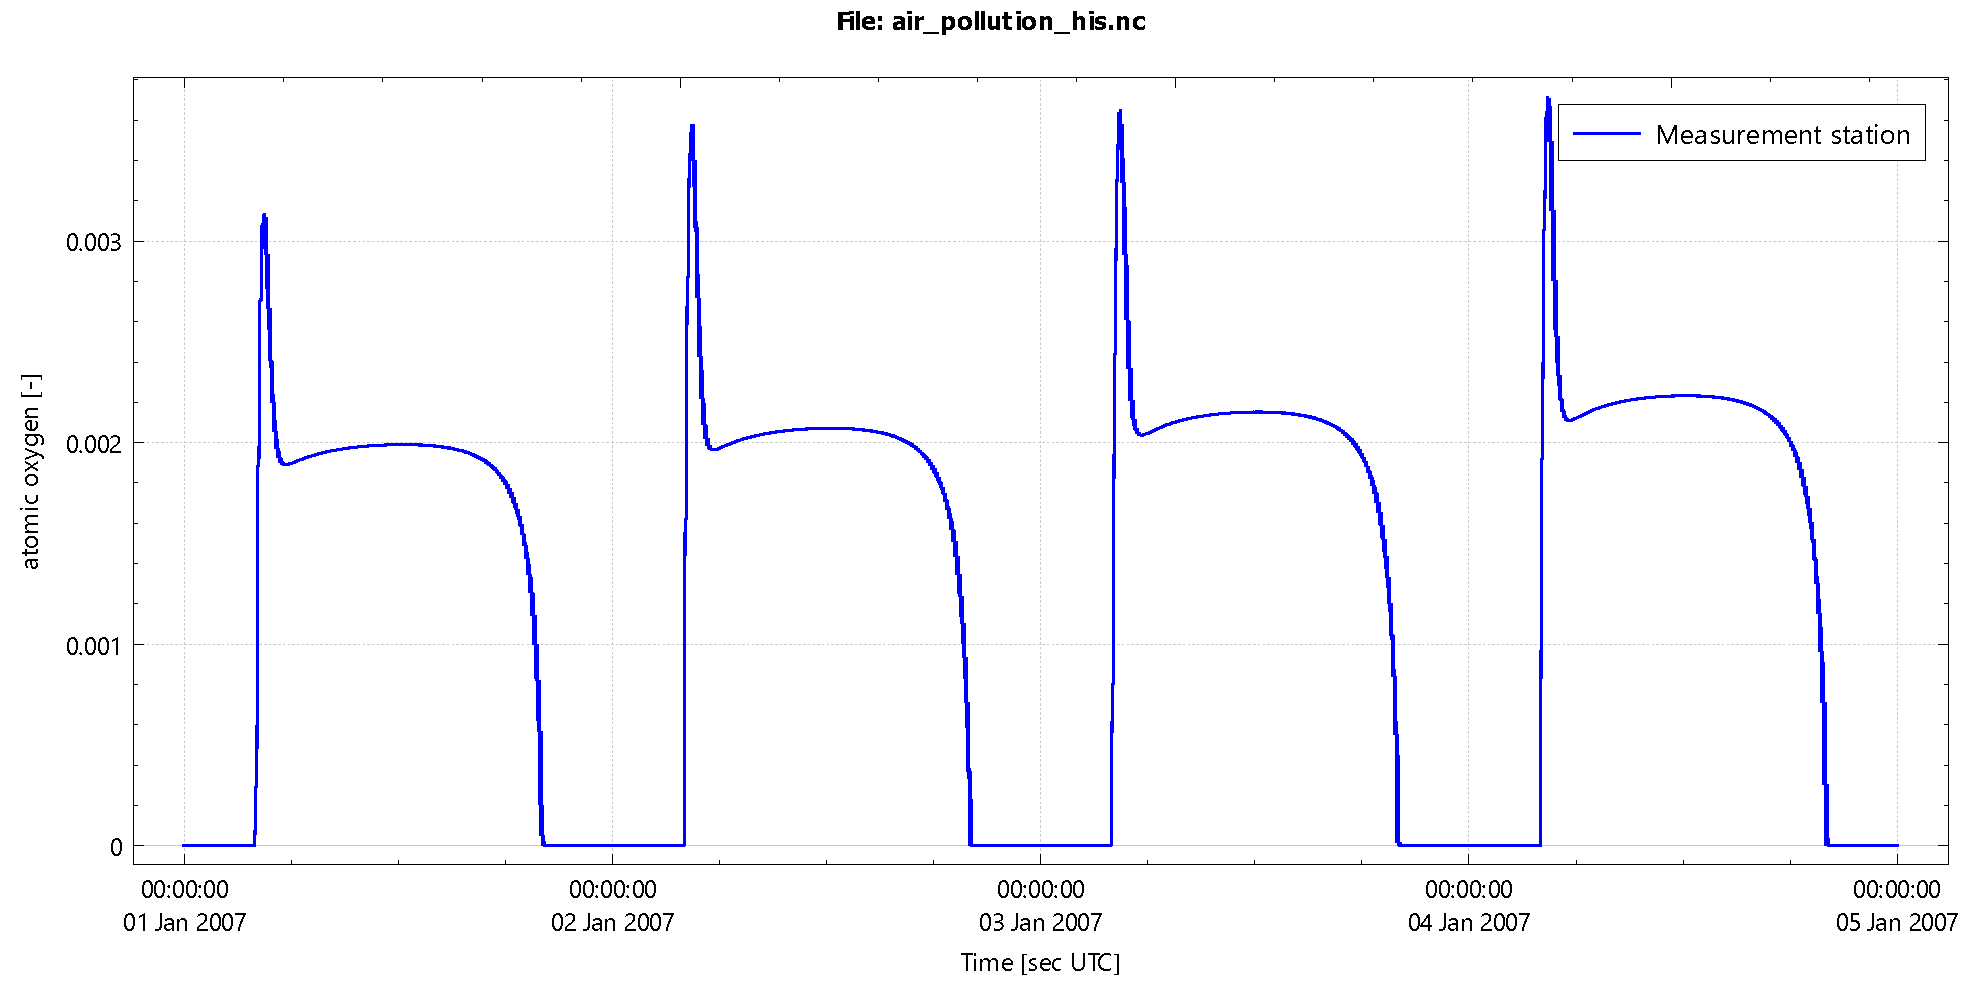
\includegraphics[width=\textwidth]{figures/atomic_oxygen_dt0d5.pdf}
        \caption{Concentration of Atomic Oxygen.}
    \end{subfigure}
    \begin{subfigure}{0.5\textwidth}
        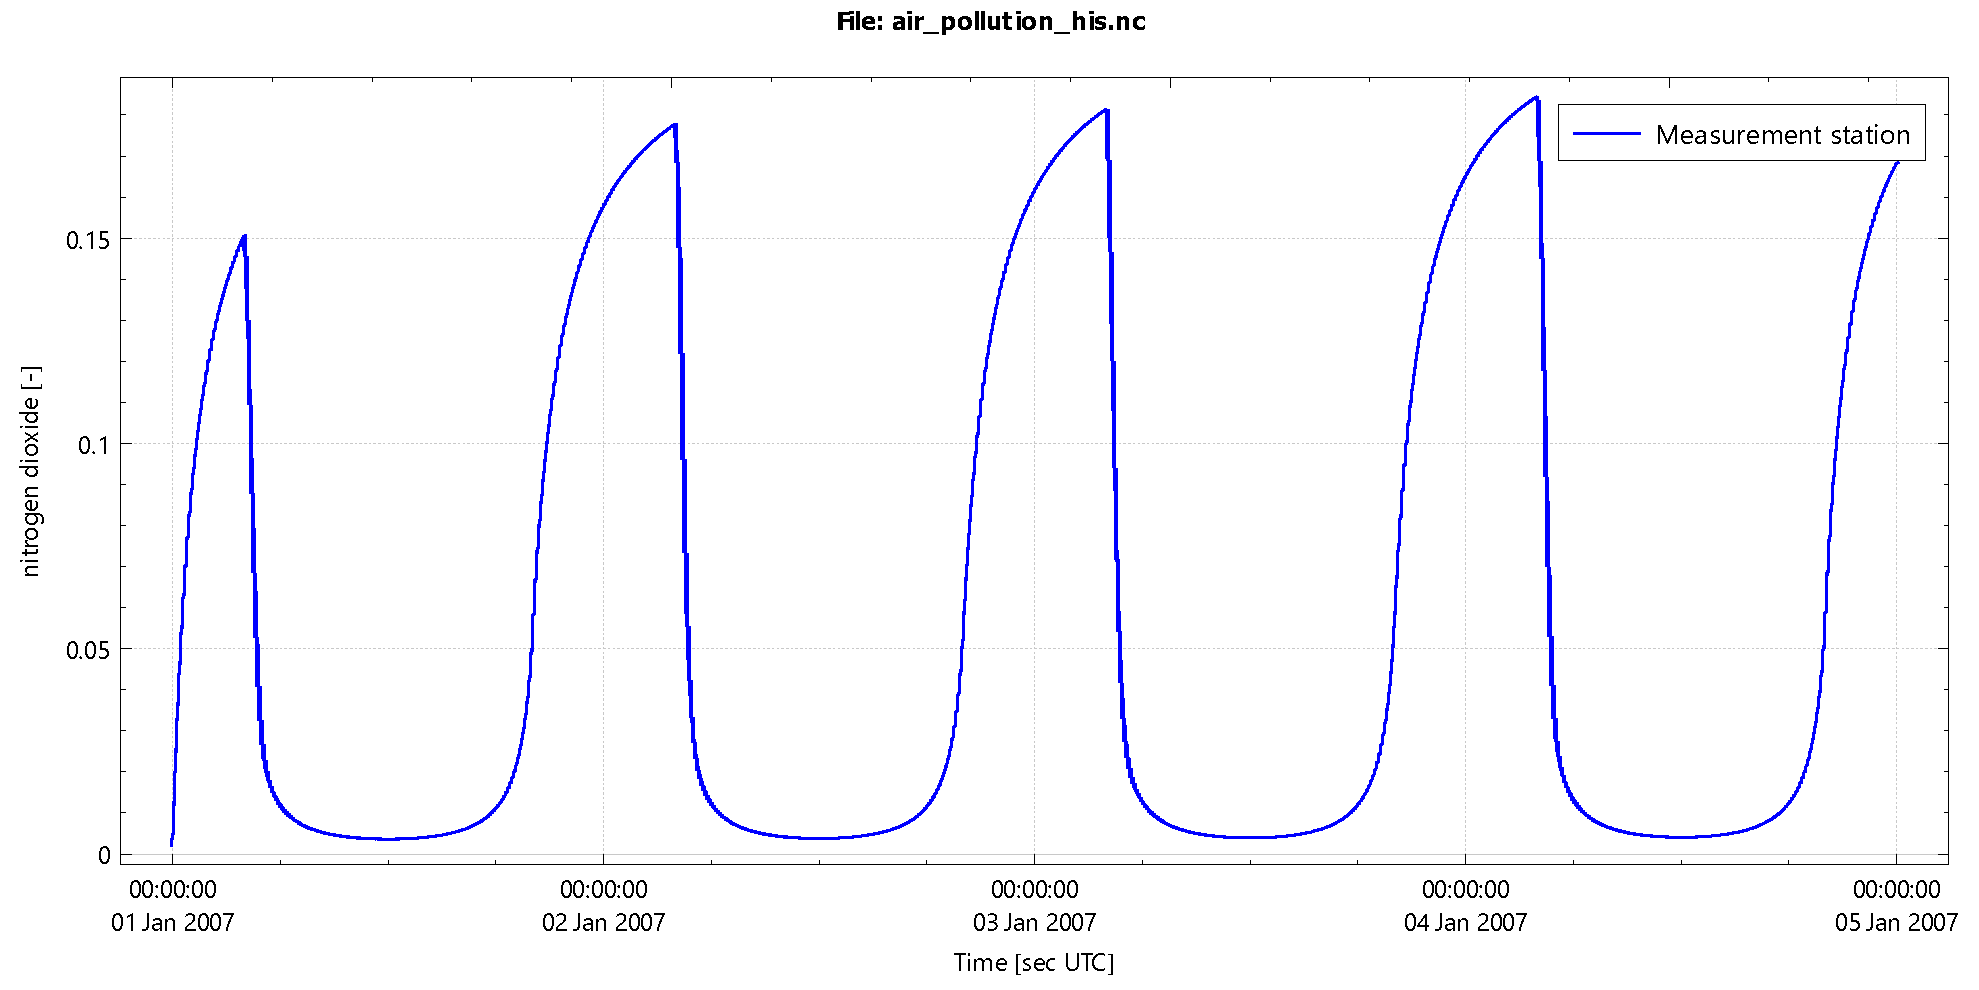
\includegraphics[width=\textwidth]{figures/nitrogen_dioxide_dt0d5.pdf}
        \caption{Concentration of Nitrogen Dioxide.}
    \end{subfigure}
    \begin{subfigure}{0.5\textwidth}
        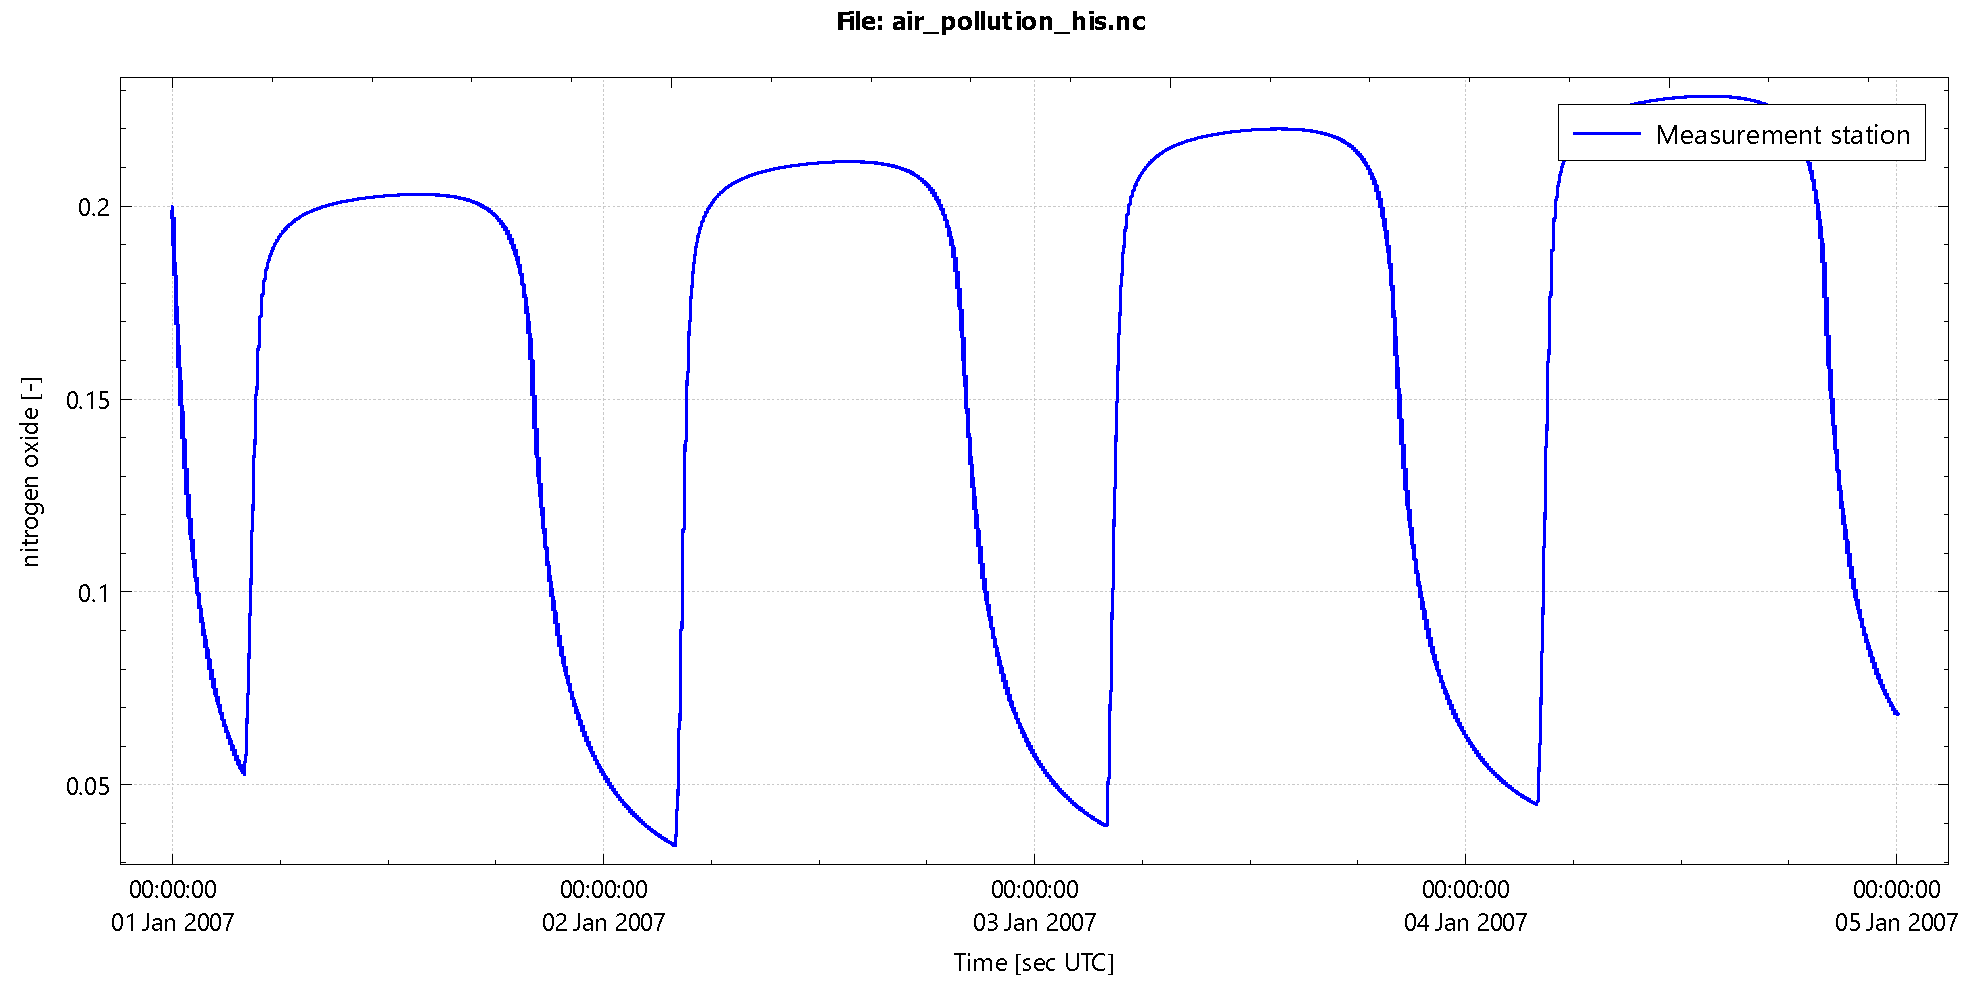
\includegraphics[width=\textwidth]{figures/nitrogen_oxide_dt0d5.pdf}
        \caption{Concentration of Nitrogen Oxide.}
    \end{subfigure}
    \begin{subfigure}{0.5\textwidth}
        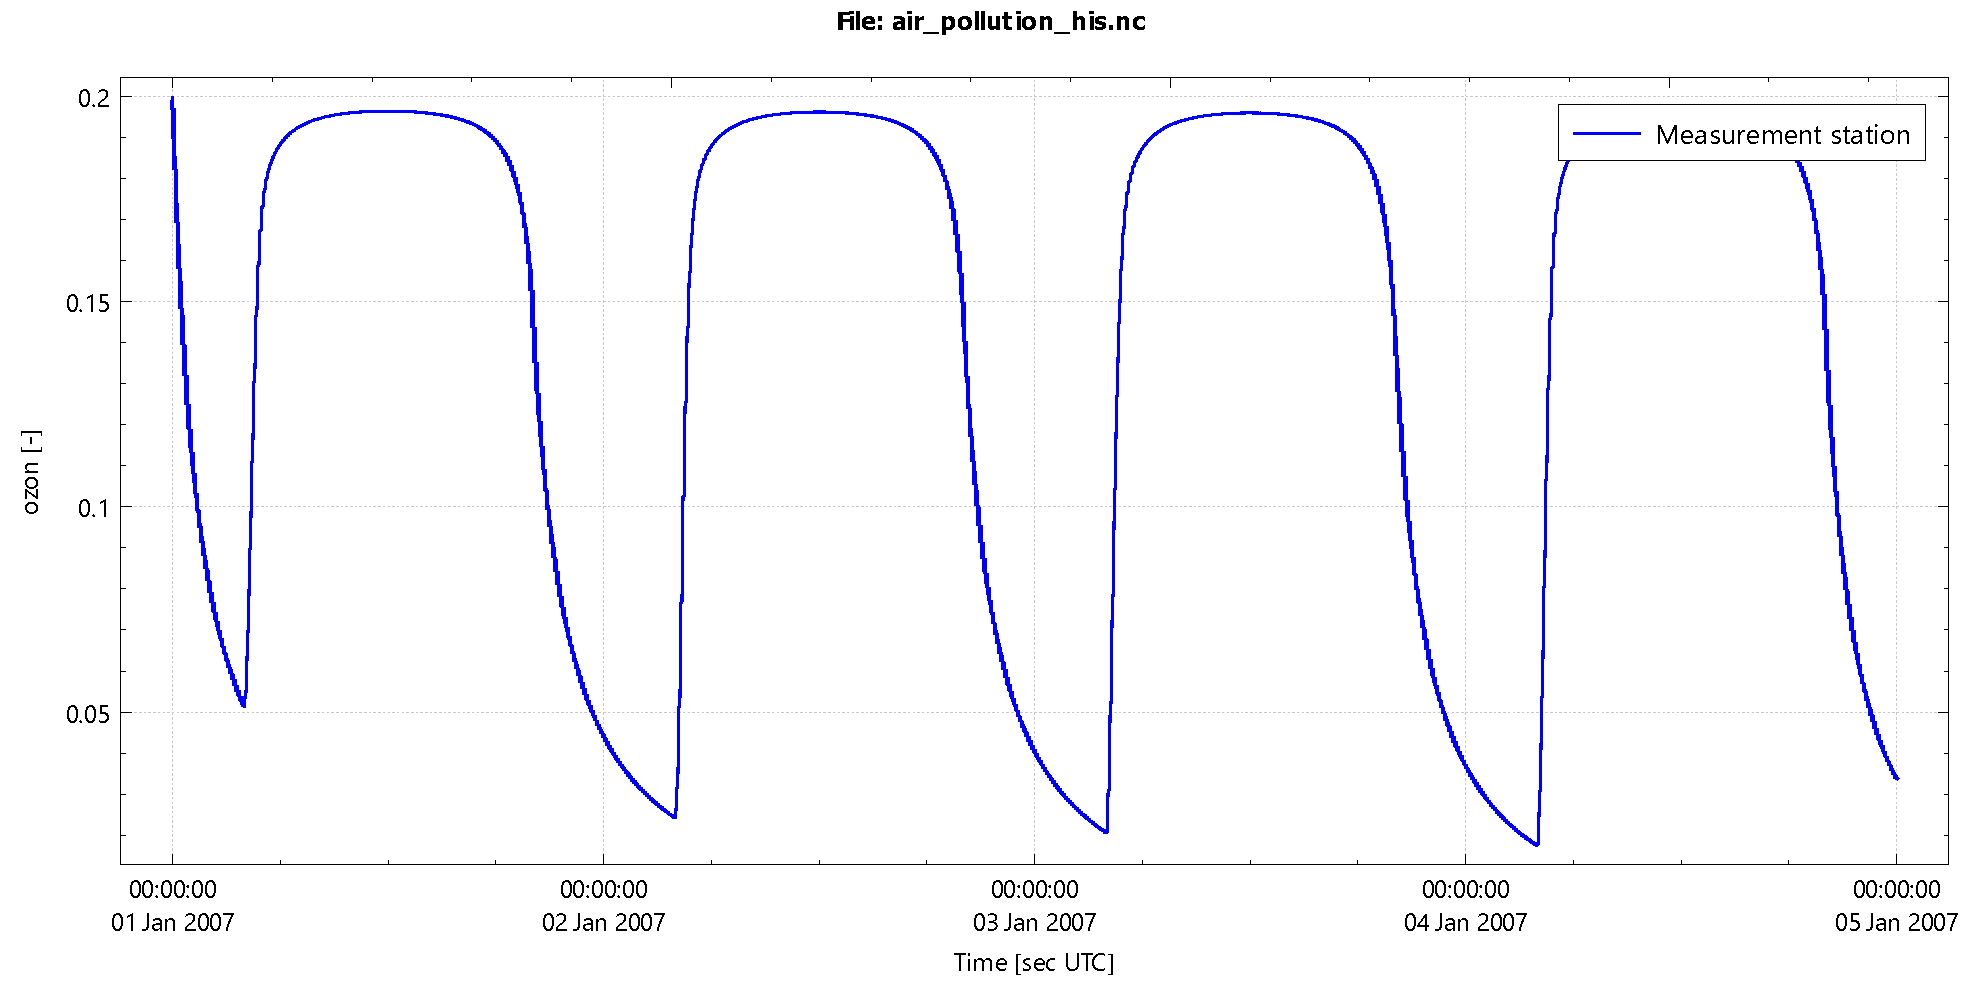
\includegraphics[width=\textwidth]{figures/ozon_dt0d5.pdf}
        \caption{Concentration of Ozon.}
    \end{subfigure}
    \caption{Result plots of the different constituents, compute with the fully implicit time integration method with a timestep of \SI{0.5}{[\second]}.}
\end{figure}

%------------------------------------------------------------------------------
\subsubsection*{Differen time integrators}
Numerical stability for different values of $\Dt$ are studied for Euler-explicit, Runga-Kutta-4 and the fully implicit $\Delta$-formulation.
%
\begin{longtable}{>{\bfseries}p{6mm-12pt}|p{\textwidth/4-2mm-12pt}|p{\textwidth/4-2mm-12pt}|p{\textwidth/4-2mm-12pt}|p{\textwidth/4-2mm-12pt}}
    \caption{Stability for different time integrators} \\%
    \rowcolor{mgreen1}
    & \textcolor{white}{\textbf{Time step\newline \si{[\second]}}}
    & \textcolor{white}{\textbf{Euler explicit}}
    & \textcolor{white}{\textbf{Runge-Kutta 4}}
    & \textcolor{white}{\textbf{Fully Implicit\newline \deltaformulation}}
    \\
    \topline
    \endfirsthead
    \rowcolor{mgreen1}
    & \textcolor{white}{\textbf{Time step\newline \si{[\second]}}}
    & \textcolor{white}{\textbf{Euler Explicit}}
    & \textcolor{white}{\textbf{Runge-Kutta 4}}
    & \textcolor{white}{\textbf{Fully Implicit\newline \deltaformulation}}
    \\
    \midline
    \endhead
    \endfoot
    \bottomline
    \endlastfoot
    1 & 0.5 & -  & \checkmark & \checkmark  \\
    \midline
    2 & 60 & \checkmark  & \checkmark  &  \checkmark \\
    \midline
    3 & 120 & Unstable & \checkmark &  \checkmark \\
    \midline
    4 & 180 & - & Unstable & \checkmark \\
    \midline
    5 & 240 & - & - & \checkmark \\
    \midline
    6 & 300 & - & - & \checkmark \\
    \midline
    7 & 900 & - & - & \checkmark \\
    \midline
    8 & 1800 & - & - & \checkmark \\
    \midline
    9 & 3600 & - & - & \checkmark \\
\end{longtable}

%
%------------------------------------------------------------------------------
\subsection{Brusselator}
%--------------------------------------------------------------------------------
Some numerical results of the brusselator example (\autoref{sec:brusselator}) is:
\begin{figure}[H]
    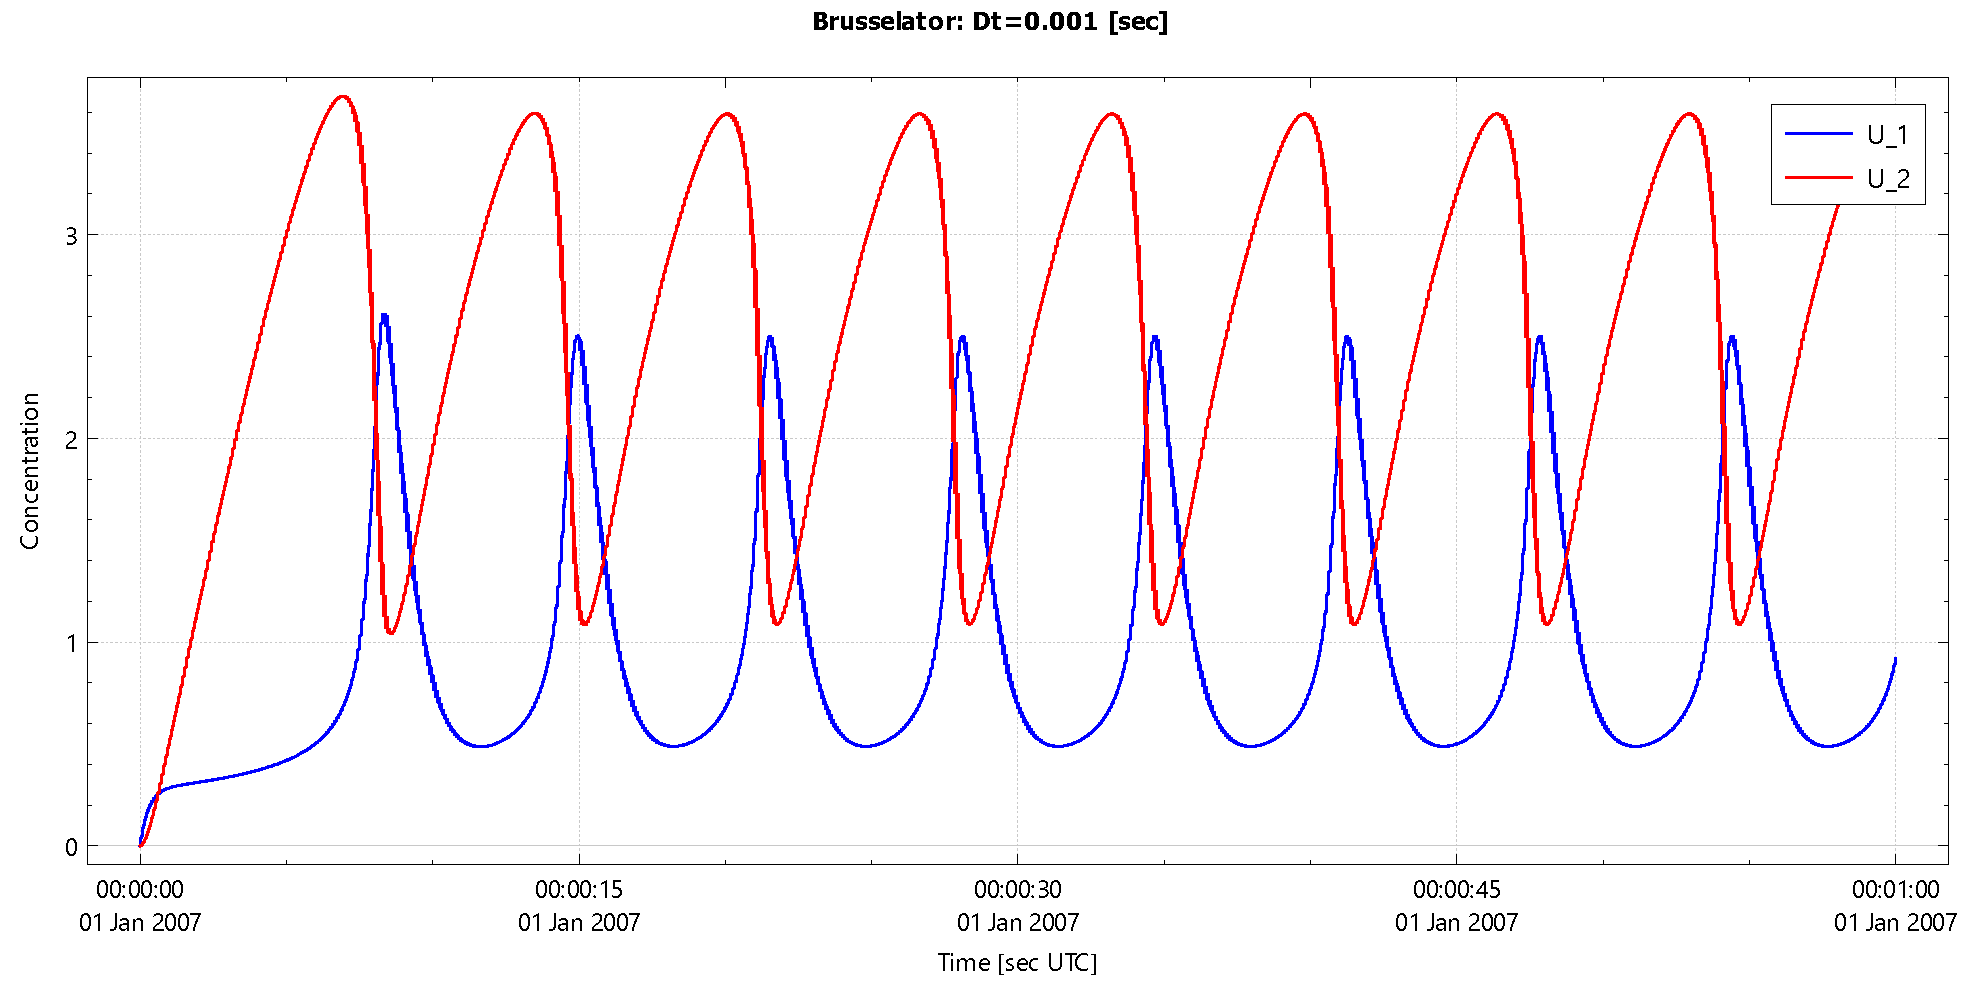
\includegraphics[width=\textwidth]{figures/brusselator_imp_dt=0d001.pdf}
    \caption{Fully Implicit: $\Dt=0.001$, $k_1=1$, $k_2=2.5$. }\label{fig:brusselator_reference}
\end{figure}
The solution presented in \autoref{fig:brusselator_reference} is assumed to be the reference (analytic) solution of \autoref{eq:brusselator}.
%
\begin{figure}[H]
    \begin{subfigure}{0.5\textwidth}
        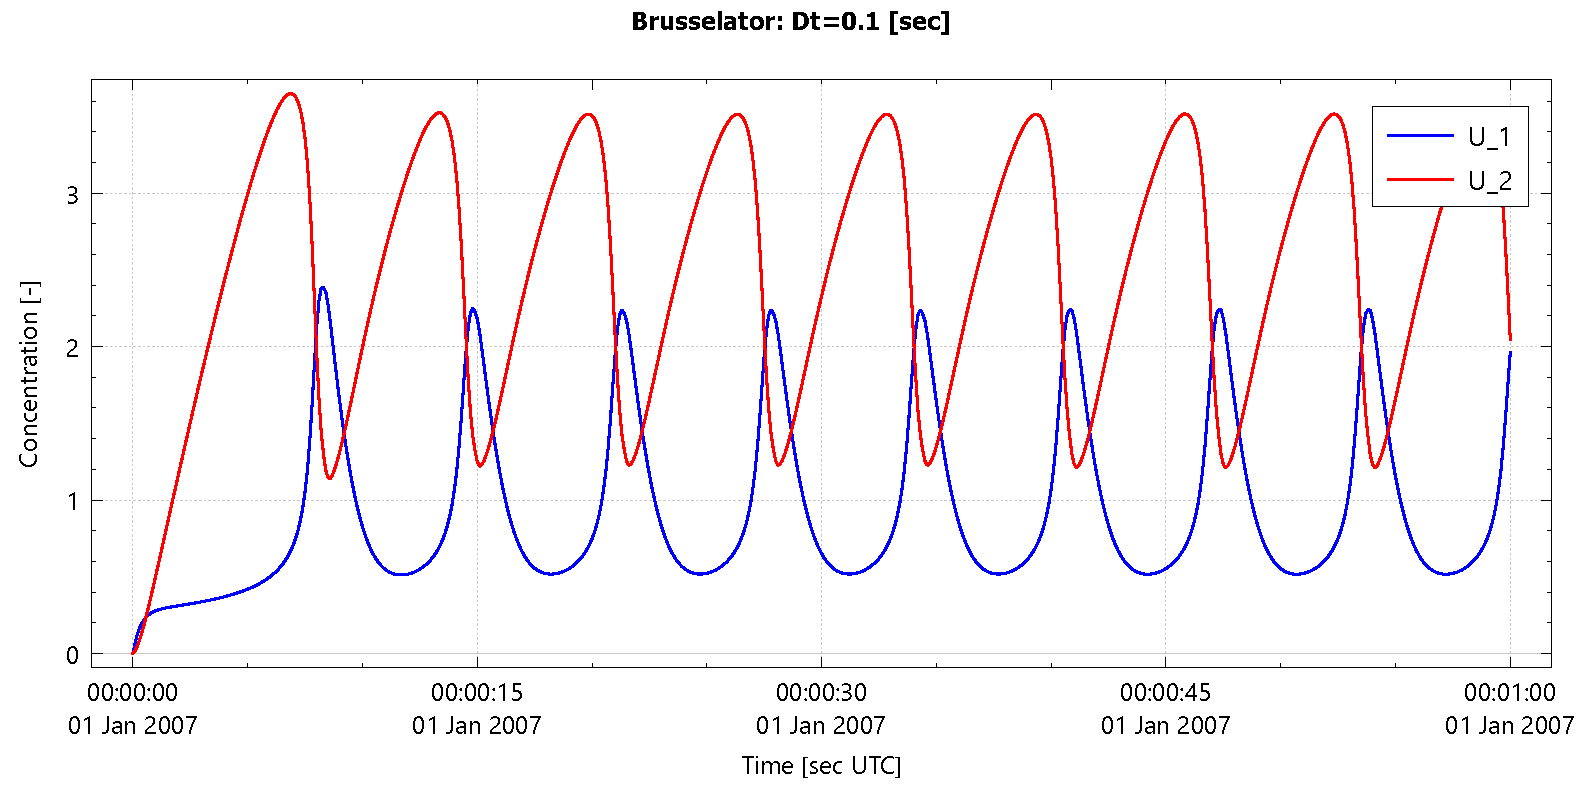
\includegraphics[width=\textwidth]{figures/brusselator_imp_dt=0d10.pdf}
        \caption{Fully Implicit: $\Dt=0.1$, $k_1=1$, $k_2=2.5$}
    \end{subfigure}
    \begin{subfigure}{0.5\textwidth}
        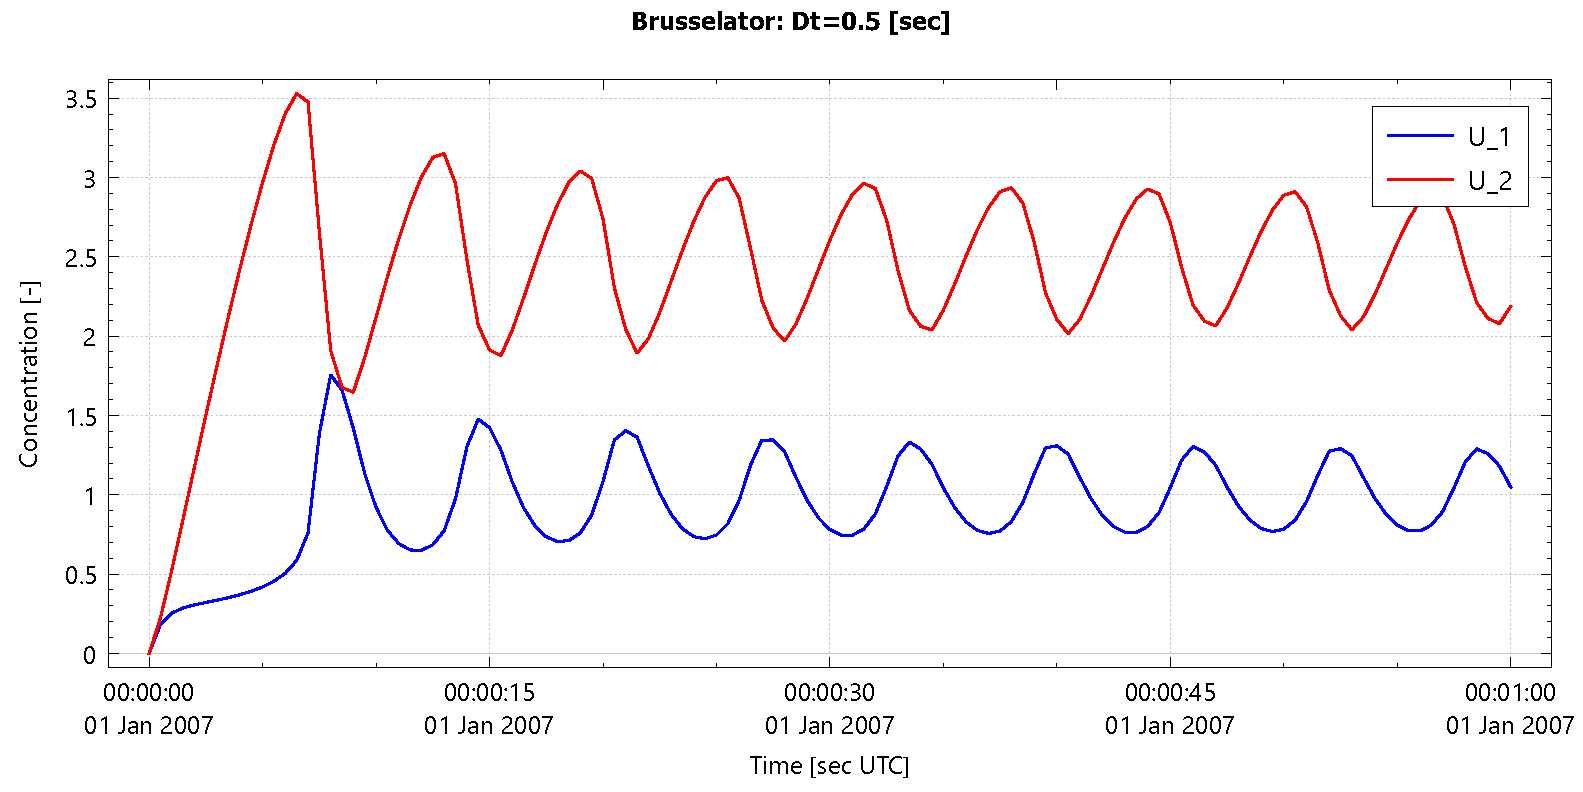
\includegraphics[width=\textwidth]{figures/brusselator_imp_dt=0d50.pdf}
        \caption{Fully Implicit: $\Dt=0.5$, $k_1=1$, $k_2=2.5$}
    \end{subfigure}
    \caption{Result plots for constant value of $k_1 = 1$ and $k_2 =2.5$, computed with a fully implicit ($\Delta$ formulation) time integration method for different time steps $\Dt = 0.001,  0.1, 0.5$.}
\end{figure}
Extra attention is needed for the Fully Implicit time integration with larger time step:
\begin{figure}[H]
    \begin{subfigure}{0.5\textwidth}
        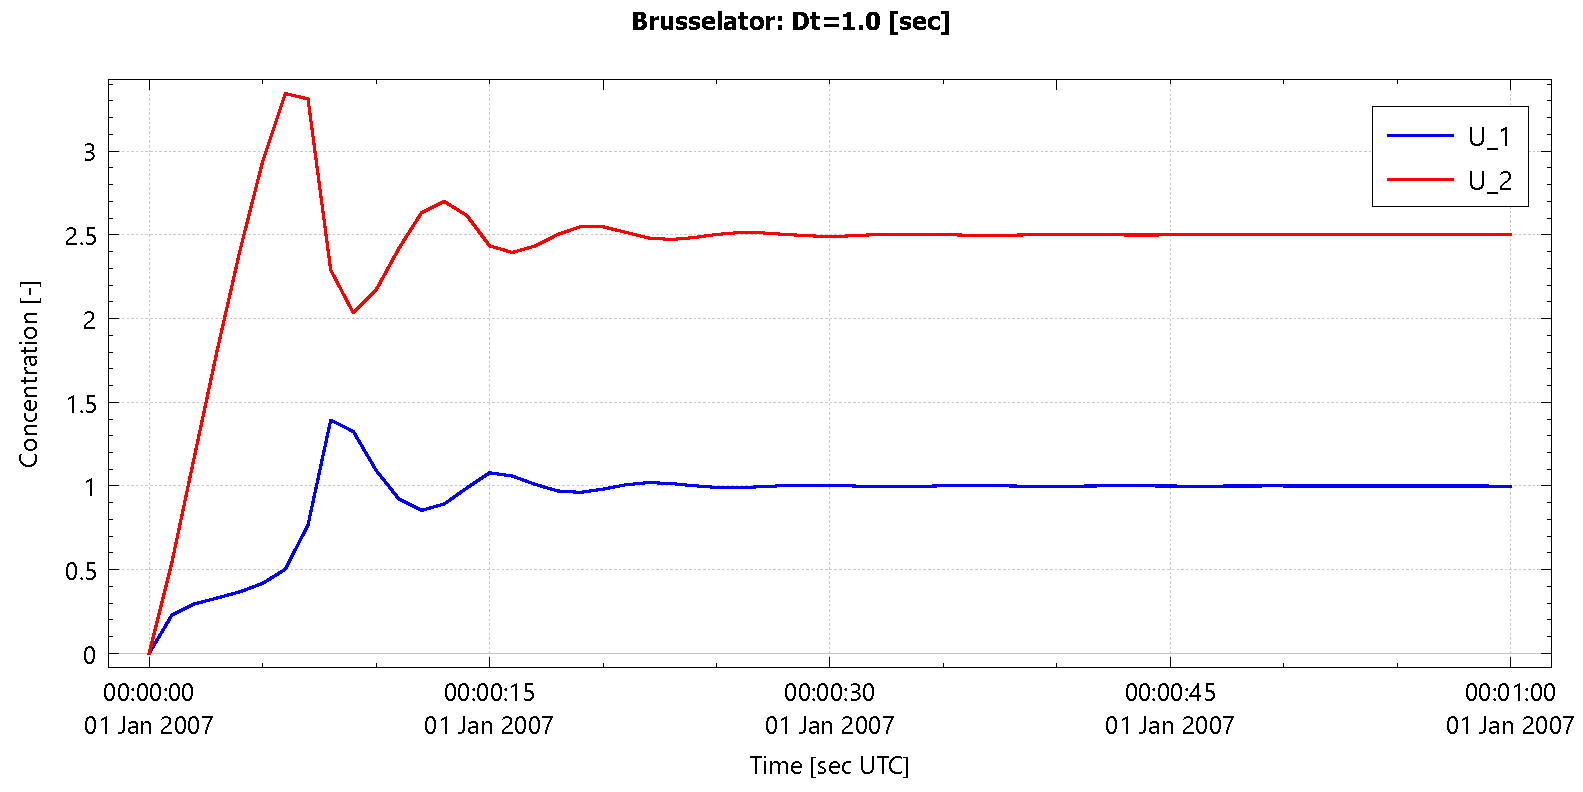
\includegraphics[width=\textwidth]{figures/brusselator_imp_dt=1d00.pdf}
        \caption{Fully Implicit: $\Dt=1.0$, $k_1=1$, $k_2=2.5$}\label{fig:imp_dt=1d00}
    \end{subfigure}
    \begin{subfigure}{0.5\textwidth}
        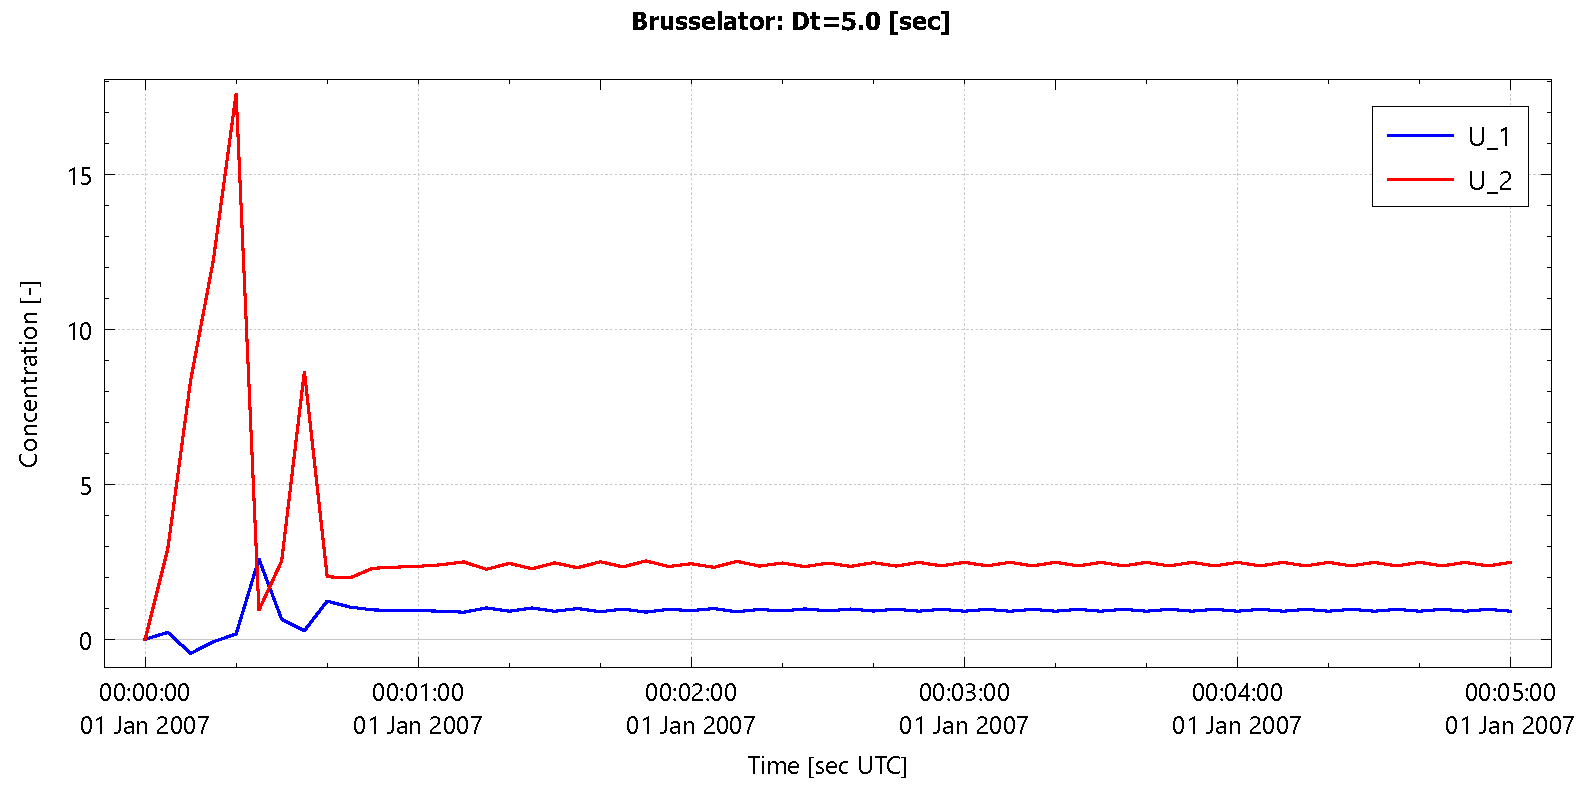
\includegraphics[width=\textwidth]{figures/brusselator_imp_dt=5d00.pdf}
        \caption{Fully Implicit: $\Dt=5.0$, $k_1=1$, $k_2=2.5$}\label{fig:imp_dt=5d00}
    \end{subfigure}
    \caption{Result plots for constant value of $k_1 = 1$ and $k_2 =2.5$, computed with a fully implicit ($\Delta$ formulation) time integration method for different time steps $\Dt = 1.0, 5.0$.
    }
\end{figure}
\Autoref{fig:imp_dt=1d00} converge to the equilibrium state $(u_1, u_2) = (1.0, 2.5)$ and
\Autoref{fig:imp_dt=5d00} looks to converge to the equilibrium state $(u_1, u_2) = (1.0, 2.5)$ but is still wiggling after \SI{5}{\minute} of simulation time (even after one day --- not presented here).
How these equations are discretized is given in \autoref{sec:brusselator_discretization}.

%------------------------------------------------------------------------------
\subsubsection*{Different time integrators}
Numerical stability for different values of $\Dt$ are studied for the Runga-Kutta-4 and fully implicit \deltaformulation.
%
\begin{longtable}{>{\bfseries}p{6mm-12pt}|p{\textwidth/3-2mm-12pt}|p{\textwidth/3-2mm-12pt}|p{\textwidth/3-2mm-12pt}}
    \caption{Stability of different time integrators for the Brusselator.} \\%
    \rowcolor{mgreen1}
    & \textcolor{white}{\textbf{Time step\newline \si{[\second]}}}
    & \textcolor{white}{\textbf{Runge-Kutta 4}}
    & \textcolor{white}{\textbf{Fully Implicit\newline \deltaformulation}}
    \\
    \topline
    \endfirsthead
    \rowcolor{mgreen1}
    & \textcolor{white}{\textbf{Time step\newline \si{[\second]}}}
    & \textcolor{white}{\textbf{Runge-Kutta 4}}
    & \textcolor{white}{\textbf{Fully Implicit\newline \deltaformulation}}
    \\
    \midline
    \endhead
    \endfoot
    \bottomline
    \endlastfoot
    1 & 0.1 & \checkmark & \checkmark  \\
    \midline
    2 & 0.2  & \checkmark &  \checkmark   \\
    \midline
    3 & 0.5 & \checkmark &  \checkmark   \\
    \midline
    4 & 1.0 & Unstable &   \checkmark  \\
    \midline
    5 & 2.0 &   &   \checkmark  \\
    \midline
    6 & 5.0 &   &   \checkmark  \\
    \midline
\end{longtable}


%--------------------------------------------------------------------------------
\section{1-D Advection equation}
The considered advection equation reads:
\begin{align}
    \pdiff{c}{t} + \pdiff{uc}{x} = 0,
\end{align}
With initial condition for the velocity $u_{given} = \SI{10}{\metre\per\second}$, which coincide with the wave celerity in the next numerical experiments.
\begin{align}
    u(x,0) = u_{given}
\end{align}
and with a prescribed boundary condition at the left side of the domain
% reg_factor = 0.5 * (std::cos(M_PI * (treg - double(nst) * dt) / treg) + 1.0);
\begin{align}
    c(0,t) = c_{given}
    \begin{cases}
        \half \cos\left(\pi \left(\frac{t_{reg} - t}{t_{reg}}\right)+ 1\right) &\quad \text{if } t < t_{reg},
        \\
        1 &\quad \text{if } t \geq t_{reg},
    \end{cases}
\end{align}
where
\begin{symbollist}
    \item[$t_{reg}$] The regularization time for the given time-series, [\si{\second}]
    \nomenclature{$t_{reg}$}{\si{\second}}{The regularization time for the given time-series}
\end{symbollist}
%--------------------------------------------------------------------------------
\subsubsection*{Numerical experiment}
The numerical experiment is performed with the following parameters:
\begin{itemize}
    \item Length of the domain, $\SI{12000}{\metre}$
    \item Grid size, $\Dx = \SI{10}{\metre}$
    \item Start time, $t_{start} = \SI{0}{\second}$
    \item End time, $t_{stop} = \SI{3600}{\second}$
    \item Timestep, $\Dt = \SI{5}{\second}$
    \item Regularization time for time-series, $t_{reg} = \SI{300}{\second}$
    \item Prescribed constant velocity, $u_{given}(x,t) = \SI{10}{\metre\per\second}$
    \item Prescribed initial value of the constituent, $c(x,0)= \SI{0}{[-]}$.
    \item Prescribed constant constituent on boundary, $c_{given}(0,t) = \SI{1}{[-]}$
\end{itemize}


%--------------------------------------------------------------------------------
\subsection{1-D Advection equation + $\mathbf{\exp(\phi)}$}
Due to numerical discretization the value $c$ could become negative, in certain applications a positive value is reguired.
To ensure the positivity of the constituent $c$ we will write the equation with variable $\phi$, where $\phi$ is defined as:
\begin{align}
    \phi = \ln(c)
\end{align}
The considered advection equation now reads:
\begin{align}
    \pdiff{\phi}{t} + \pdiff{u\phi}{x} = 0,\label{eq:1d_advec_phi}
\end{align}
With initial condition for the velocity $u_{given} = \SI{10}{\metre\per\second}$, which coincide with the wave celerity in the next numerical experiments.
\begin{align}
    u(x,0) = u_{given}
\end{align}
and with a prescribed boundary condition for the constituent $c$ at the left side of the domain
\begin{align}
    c(0,t) = c_{given}
    \begin{cases}
        \half \cos\left(\pi \left(\frac{t_{reg} - t}{t_{reg}}\right)+ 1\right) &\quad \text{if } t < t_{reg},
        \\
        1 &\quad \text{if } t \geq t_{reg},
    \end{cases}
\end{align}
where
\begin{symbollist}
    \item[$t_{reg}$] The regularization time for the given time-series, [\si{\second}]
    \nomenclature{$t_{reg}$}{\si{\second}}{The regularization time for the given time-series}
\end{symbollist}
A value of $c(0,t)=0$ is estimated by, so:
\begin{align}
    \phi(0,t) = \ln(c(0,t)) \gtrsim -50
\end{align}
%--------------------------------------------------------------------------------
\subsubsection*{Numerical experiment}
The numerical experiment is performed with the following parameters:
\begin{itemize}
    \item Length of the domain, $\SI{12000}{\metre}$
    \item Grid size, $\Dx = \SI{10}{\metre}$
    \item Start time, $t_{start} = \SI{0}{\second}$
    \item End time, $t_{stop} = \SI{3600}{\second}$
    \item Timestep, $\Dt = \SI{5}{\second}$
    \item Regularization time for time-series, $t_{reg} = \SI{300}{\second}$
    \item Prescribed constant velocity, $u_{given}(x,t) = \SI{10}{\metre\per\second}$
    \item Prescribed initial value of the constituent, $c(x,0)= \num{1e-20}$, \newline so $\phi = \SI{-50}{[-]}$.
    \item Prescribed constant constituent on boundary $c_{given}(0,t) = 1$, \newline so $\phi = \ln(c_{given}(0,t)) = \ln(1) = \SI{0}{[-]}$
\end{itemize}
%--------------------------------------------------------------------------------
\section{1-D Wave equation}
The considered 1-D wave equation reads:
\begin{align}
    \pdiff{h}{t}  + \pdiff{q}{x} & = 0 \qquad \textit{continuity eq.} \\
    \pdiff{q}{t}  + g h \pdiff{h}{x} & = 0 \qquad \textit{momentum eq.}
\end{align}
With initial conditions
\begin{align}
    h(x,0) & = \zeta(x,0) - z_b(x),\\
    q(x,0) & = 0
\end{align}
for the the water level a Gaussian hump is prescribed
\begin{align}
    \zeta(x) = 2 a_0 \exp\left( \frac{(x - \mu)^2}{2\sigma^2}  \right), \quad [\si{\metre}]
\end{align}
At the boundaries no ingoing signals are prescribed, so outgoing signals are leaving the domain unhampered, which means no reflections will be present other then numerical reflections.

The numerical experiment is performed with the following parameters:
\begin{itemize}
    \item Length of the domain, $\SI{12000}{\metre}$, ranging from $\SI{-6000}{\metre}$ to $\SI{6000}{\metre}$.
    \item Bed level, $z_b = \SI{-10}{\metre}$.
    \item Grid size, $\Dx = \SI{10}{\metre}$.
    \item Start time, $t_{start} = \SI{0}{\second}$.
    \item End time, $t_{stop} = \SI{3600}{\second}$.
    \item Timestep, $\Dt = \SI{10}{\second}$.
    \item Regularization time for time-series, $t_{reg} = \SI{300}{\second}$.
    \item Amplitude of the Gaussian hump at the boundary, $a_0 = \SI{0.01}{\metre}$.
    \item Centre of the Gaussian hump, $\mu = \SI{3000}{\metre}$.
    \item Spreading of the Gaussian hump, $\sigma = \SI{700}{\metre}$.
\end{itemize}
And an experiment with given boundary values:
\begin{itemize}
    \item Prescribed discharge boundary at $\SI{-6000}{\metre}$: $q(0,t) = \SI{0.05}{\square\metre\per\second}$.
    \item Prescribed water level boundary value at $\SI{6000}{\metre}$: $\zeta(0,t) = \SI{0.02}{\metre}$.
\end{itemize}
Because the boundary values are constant in time the solution is time-independent.
Therefore two simulation should be performed:
\begin{enumerate}
    \item A stationary computation (with $\Dt = \SI{0}{\second}$) and
    \item an temporal computation (with $t_{stop} = \SI{10800}{\second}$)
\end{enumerate}
